\documentclass[10pt,twocolumn]{article}
\usepackage[letterpaper,margin=0.55in,columnsep=0.24in]{geometry}
\usepackage{times}
\usepackage{amsmath,amssymb}
\usepackage{graphicx}
\graphicspath{{figs/}}
\usepackage[numbers,sort&compress]{natbib}
\usepackage{hyperref}
\usepackage{titlesec}
\usepackage{caption}
\usepackage{enumitem}
\usepackage{booktabs}
\usepackage{xcolor}
\captionsetup{font=footnotesize, skip=4pt}
\setlength{\textfloatsep}{6pt plus 1pt minus 1pt}
\setlength{\intextsep}{6pt plus 1pt minus 1pt}
\setlength{\floatsep}{4pt plus 1pt minus 1pt}

\hypersetup{colorlinks=true, linkcolor=black, citecolor=black, urlcolor=blue}

% ---- IEEE-like section styling ----
\titleformat{\section}{\normalfont\centering\normalsize\bfseries}{\Roman{section}.}{0.6em}{\MakeUppercase}
\titleformat{\subsection}{\normalfont\itshape}{\Alph{subsection}.}{0.5em}{}
\titlespacing*{\section}{0pt}{1.2em}{0.6em}
\titlespacing*{\subsection}{0pt}{0.8em}{0.4em}

\newcommand{\papertitle}{NBA Career Longevity: What Predicts How Long a Player Lasts in the League?}

\title{\papertitle}
\author{
  Eilam Spivak, Asaf Buzaglo \\
  \small Department of Statistics, Bar-Ilan University \\
  \small I.D.: 216602037, 331734053 \\
  \small Email: \texttt{eylamspivak@gmail.com}, \texttt{asafb4@gmail.com}
}
\date{}

\begin{document}
\twocolumn[
  \maketitle
  \begingroup
  \centering
  \parbox{0.92\textwidth}{\small
    \textbf{Code and data:}
    \url{https://github.com/eylamspivak/statistical-theory-final-project}
  }
  \vspace{0.6em}

  \parbox{0.92\textwidth}{\small
    \textbf{Abstract---}
    This study investigates what predicts the career longevity of
    National Basketball Association (NBA) players, using an incident
    cohort of \textbf{2{,}110} rookies whose debut season is confirmed
    within the 1997--2022 window of the dataset (441 players whose
    first \emph{recorded} season coincided with the dataset's own
    first season were excluded, since a true rookie season could not
    be confirmed for them). High-scoring rookies had significantly
    longer careers than low-scoring rookies (Welch $t=14.06$,
    $p<0.0001$, Cohen's $d=0.61$). Career length differed sharply by
    draft round (Round-1 mean 7.49 seasons vs.\ 4.38 for Round-2 vs.\
    3.22 undrafted; ANOVA $F=236.8$, $p<0.0001$, confirmed by
    Kruskal--Wallis after Levene's test revealed unequal variances).
    Draft age was negatively associated with career length
    ($r=-0.294$, $p<0.0001$). Critically, when rookie-season attributes
    and draft round were entered into a single nested-model comparison,
    both contributed statistically independent explanatory power
    (nested $F$-tests / GLRT, both $p<0.0001$): $R^2$ rose from 0.203
    (rookie attributes only) and 0.184 (draft round only) to 0.251
    combined --- directly confirming, on a modern cohort, the sunk-cost
    pattern documented by \citet{staw1995sunk}. A logistic classifier
    distinguishing short from long careers, using the same combined
    feature set, reached \textbf{66.1}\% accuracy
    against a \textbf{50.7}\% majority-class baseline
    (AUC$=0.719$). A 1000-simulation Wald
    sequential test supported the PPG effect in 77.8\% of simulations,
    consistent with the $t$-test result. Together, these results
    indicate that both circumstantial factors fixed at draft time and
    controllable on-court performance
    independently predict NBA career length.
  }
  \par
  \endgroup
  \vspace{0.8em}
]

% ════════════════════════════════════════════════════════════
\section{Introduction}
% ════════════════════════════════════════════════════════════

The National Basketball Association (NBA) is the premier professional
basketball league in North America, comprising 30 teams that each play an
82-game regular season. Every year, a player's performance is summarized
by per-game statistics such as \textbf{points per game (PPG)},
\textbf{rebounds per game (RPG)}, and \textbf{assists per game (APG)} ---
the average number of points scored, rebounds collected, and passes
leading directly to a basket, respectively, across all games a player
appeared in that season. A player's first season in the league is
referred to as their \textit{rookie season}.

New talent enters the league primarily through the \textbf{NBA Draft}, an
annual event in which teams take turns selecting eligible players, most
commonly from American college basketball or international leagues. Since
1989 the draft has consisted of exactly two rounds of 30 picks each
(60 players total) \citep{sleeper2024draft}. Being selected in
\textbf{Round 1} is generally considered a stronger signal of a team's
confidence in a player than being selected in \textbf{Round 2}, and some
eligible players are not selected at all --- they remain
\textbf{undrafted}, and may still join a team afterward, typically with a
less secure roster spot. This draft outcome is fixed at the very start of
a player's career and is determined by scouts' evaluations of amateur or
international performance, not by anything the player has yet done in the
NBA itself.

A player's \textbf{career length} --- the number of distinct NBA seasons
in which they appear --- is a natural measure of professional success and
durability. Career longevity carries practical consequences for players
(career earnings, pension eligibility), teams (roster planning, contract
risk), and the league more broadly. Yet it is not obvious in advance
which factors matter most: does on-court production predict staying
power, or do off-court signals fixed at draft time --- such as being a
high draft pick, or entering the league at a young age --- dominate
instead?

\subsection{Related Work}
This question has a history in sports economics. \citet{staw1995sunk}
found that draft order predicts NBA playing time and survival
\textit{even after controlling for performance}, interpreted as a
sunk-cost/escalation-of-commitment effect. \citet{groothuis2004exit}
confirm this using formal duration (survival) analysis.
\citet{fynn2012analysis} apply Kaplan--Meier, Cox proportional-hazards,
and accelerated-failure-time models directly to NBA career length,
finding height and awards extend careers. We revisit this question on
a more recent cohort (1997--2022) and, following the sunk-cost
literature's core method, explicitly test whether performance and
draft position each carry independent explanatory power in the
\textit{same} model (Section~\ref{sec:results}), rather than separately.

In this project we ask: \textit{Can we predict how long an NBA player's
career will last based on their rookie-season performance, and which
factors --- performance-based and circumstantial --- drive that outcome?}
We break this broad question into four testable hypotheses:

\begin{itemize}[leftmargin=1.4em]
  \item \textbf{H1:} Players who score more points per game in their
  rookie season have significantly longer careers than lower-scoring
  players.
  \item \textbf{H2:} Career length differs significantly by draft round
  (Round~1 vs.\ Round~2 vs.\ undrafted).
  \item \textbf{H3:} Age at a player's first NBA season is negatively
  associated with career length.
  \item \textbf{H4:} Performance (H1) and draft round (H2) each carry
  explanatory power for career length \textit{independent} of the
  other, when tested jointly in the same model (directly following
  \citet{staw1995sunk} and \citet{groothuis2004exit}).
\end{itemize}

\subsection{Dataset}
Our data is drawn from the \textit{NBA Players Data} dataset on Kaggle
\citep{kaggle2024nbadata}, which contains one row per player per season,
covering NBA seasons from 1996--97 through 2021--22. Each row includes 21
fields describing that player's performance and biographical information
for that season, including points, rebounds, and assists per game;
advanced metrics such as net rating, usage percentage, true shooting
percentage, and assist percentage; physical attributes (height, weight,
age); and draft information (round, pick number, year).

\textbf{Incident-cohort filtering.} The dataset's coverage begins at the
1996--97 season, but many players active in that first season had
already begun their careers earlier, outside the data's window. Naively
taking each player's earliest \emph{recorded} row as their ``rookie
season'' would misclassify these veterans as young rookies, corrupting
age-at-entry and any variable derived from it. We therefore restrict
the analytic sample to the \textit{incident cohort}: players whose
first recorded season is strictly after 1996--97, for whom we can
confirm the recorded first season genuinely was their NBA debut. We
report how many players this excludes in Section~\ref{sec:results}.

From the remaining player-season data we derive two key variables: (i)
\texttt{career\_length}, defined as the span (in seasons) from a
player's first to last appearance in the dataset, inclusive --- we
verified this against the alternative definition of counting only
distinct seasons played (which differs only for players with a gap
season, e.g.\ due to injury or an overseas stint) and report the
number of affected players in Section~\ref{sec:results} --- and (ii)
each player's \textit{rookie-season} record, obtained by taking their
earliest season's row. All subsequent analysis is performed at the
player level, using rookie-season statistics to predict eventual
career length.

\subsection{Roadmap}
Section~\ref{sec:results} presents our results in the order the analysis
was conducted: from cleaning and describing the data, through testing
each hypothesis individually, to a combined regression, nested-model
comparison, and classification model with cross-validation.
Section~\ref{sec:methods} details the statistical methods used.
Section~\ref{sec:discussion} discusses limitations and directions for
further work.

% ════════════════════════════════════════════════════════════
\section{Results}
\label{sec:results}
% ════════════════════════════════════════════════════════════

\subsection{Data Overview and the Distribution of Career Length}
After applying the incident-cohort filter, our sample contains
\textbf{2{,}110 players} (\textbf{441} players were excluded for
having their first recorded season coincide with the dataset's first
season, 1996--97), with career length ranging from 1 to 25 seasons
(mean $=5.13$, median $=4.00$, SD $=4.36$). As Fig.~\ref{fig:dist}
shows, the distribution is right-skewed (skewness $=1.11$). Within
this 2{,}110-player analytic sample, the two \texttt{career\_length}
definitions (span vs.\ distinct-season-count) differ for
\textbf{297} players (those with a gap season);
we use span throughout for consistency with the paper.

\begin{figure}[htbp]
  \centering
  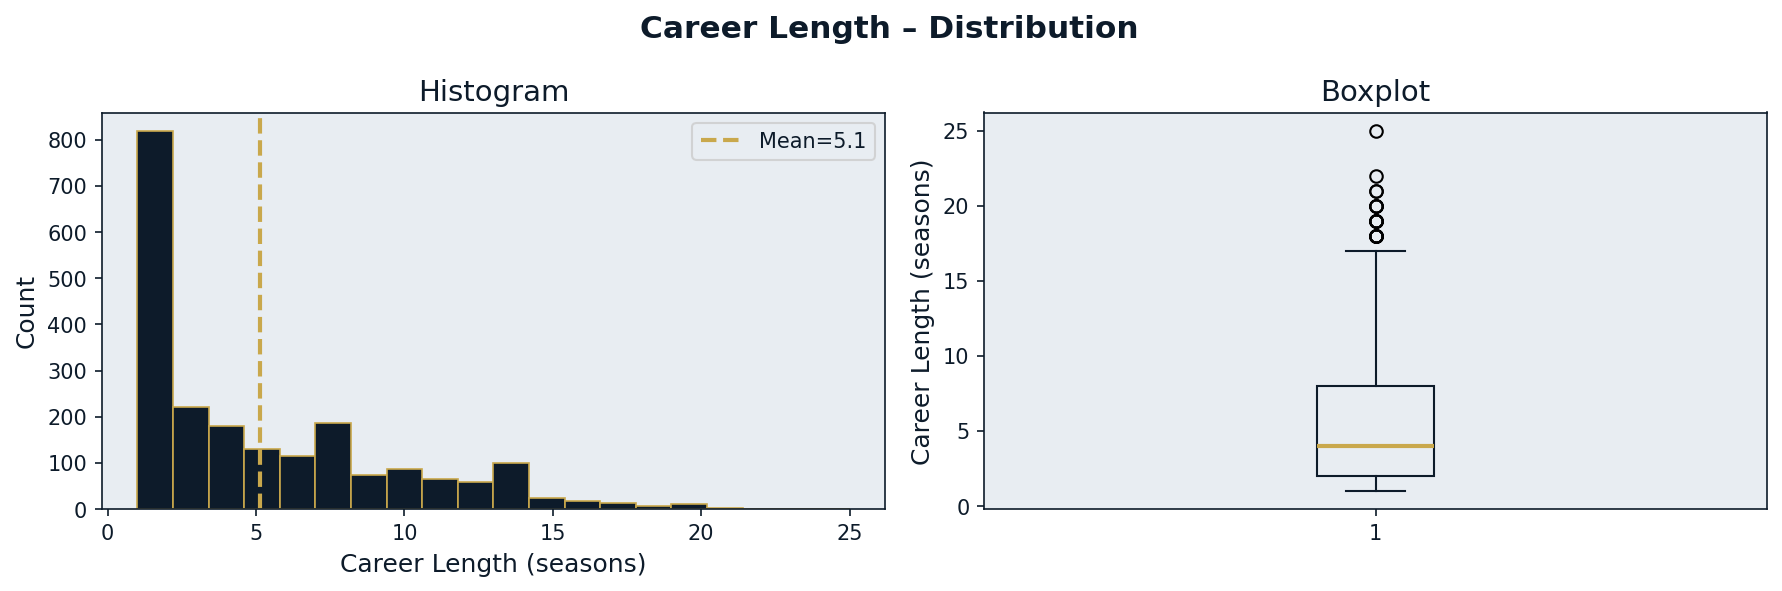
\includegraphics[width=\linewidth]{fig1_distribution.png}
  \caption{Distribution of career length: histogram (left) and boxplot (right).}
  \label{fig:dist}
\end{figure}

\subsubsection{Goodness-of-Fit}
The Kolmogorov--Smirnov test against a Normal distribution
($D=0.180$, $p<0.0001$) and the Shapiro--Wilk test ($W=0.856$,
$p<0.0001$) both indicate career length is not normally distributed
(though the KS result should be treated as indicative only, since its
parameters were estimated from the same sample --- the Lilliefors
problem). Because \texttt{career\_length} is a small positive integer
with many ties, we treat a \textbf{discrete $\chi^2$ goodness-of-fit
test} (Fig.~\ref{fig:qq}), grouping exact integer values with
infinite-tailed end categories, as the primary GOF result:
$\chi^2=386.5$, $df=5$, $p<0.0001$ --- normality is decisively
rejected. We additionally fit a \textbf{Geometric distribution} by MLE
($\hat p=0.195$, implied median survival $\approx3.2$ seasons) as a
natural ``constant hazard'' model for career length, and test its fit
with the same grouped $\chi^2$ approach (Fig.~\ref{fig:geom}):
$\chi^2=73.3$, $df=6$, $p<0.0001$ --- the geometric model is also
rejected. Rather than inferring hazard behavior indirectly from this
test alone, Fig.~\ref{fig:hazard} plots the \textbf{empirical hazard
rate} $\hat h(k) = \#\{L=k\}/\#\{L\ge k\}$ directly against the
constant hazard the geometric model assumes, and shows exactly why:
the hazard follows a \textbf{U-shape (``bathtub'') pattern}, starting
high at $k=1$ ($\hat h=0.24$, likely players who do not make an NBA
roster beyond their rookie deal), declining to a minimum around
$k=5$--$7$ ($\hat h\approx0.14$--$0.15$, established players), then
rising steadily through the later seasons ($\hat h=0.22$--$0.25$ by
$k=10$--$13$, and $\hat h=0.42$ at $k=14$, though this final point
rests on a small risk set of only 132 players and should be treated
cautiously). This directly motivates the Kaplan--Meier / hazard-based
approach discussed in Section~\ref{sec:discussion}.

\begin{figure}[htbp]
  \centering
  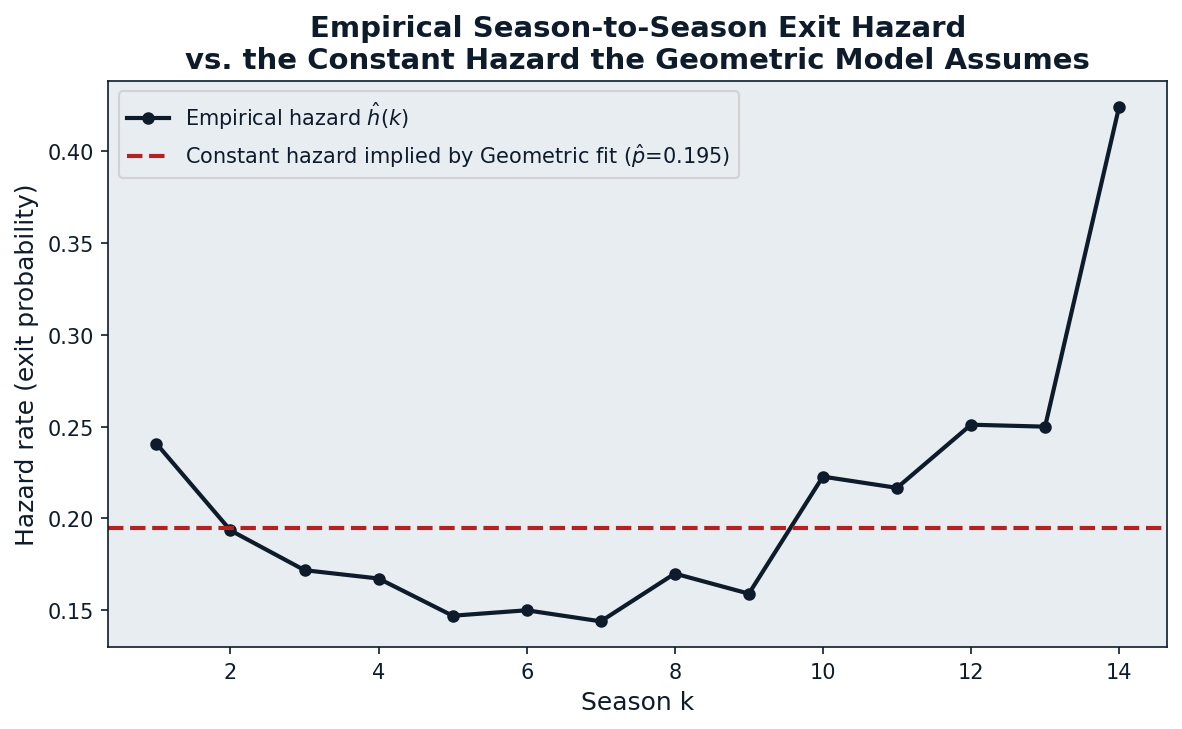
\includegraphics[width=\linewidth]{fig18_hazard.png}
  \caption{Empirical season-to-season exit hazard vs.\ the constant
  hazard implied by the Geometric MLE fit.}
  \label{fig:hazard}
\end{figure}

\begin{figure}[htbp]
  \centering
  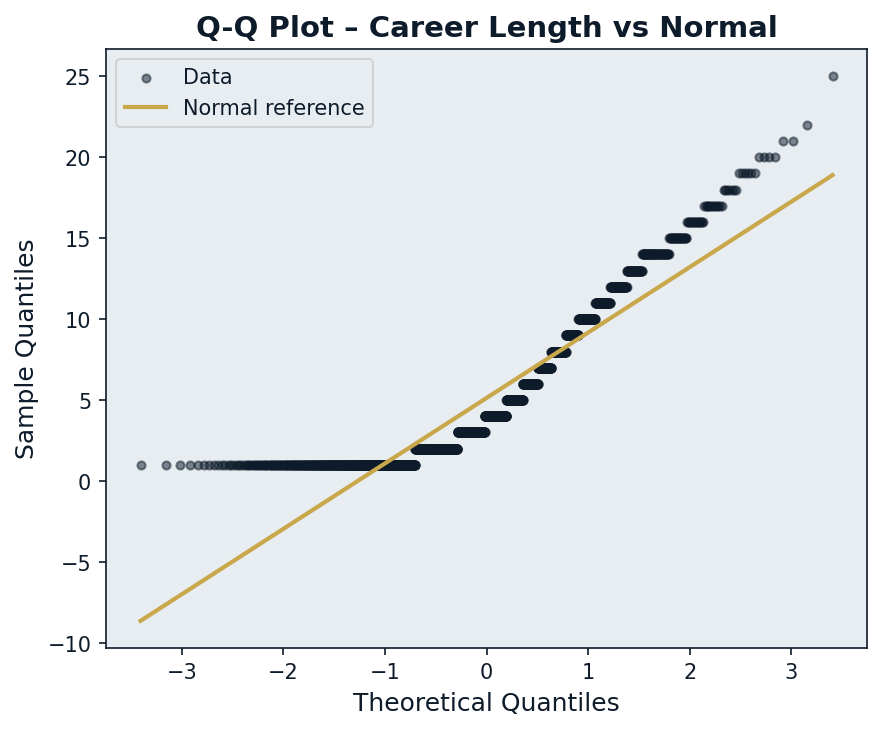
\includegraphics[width=0.49\linewidth]{fig2_qqplot.png}\hfill
  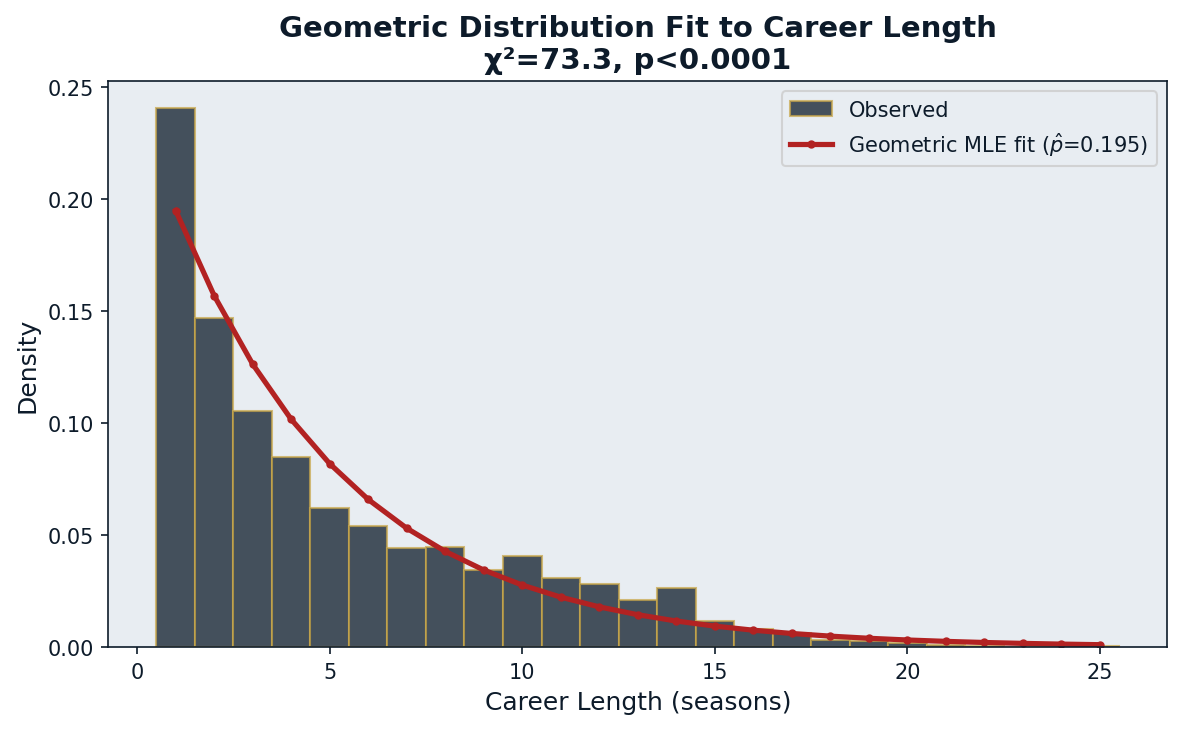
\includegraphics[width=0.49\linewidth]{fig15_geometric_fit.png}
  \caption{Left: Q-Q plot of career length vs.\ Normal. Right:
  Geometric-distribution MLE fit.}
  \label{fig:qq}
  \label{fig:geom}
\end{figure}

\subsection{H1: Rookie Scoring and Career Length}
Splitting players at the median rookie-season PPG (3.8), high-scoring
rookies ($n=1064$) averaged \textbf{6.39} seasons compared to
\textbf{3.85} for low-scoring rookies ($n=1046$). A one-sided
\textbf{Welch} $t$-test (unequal variances) confirms this difference:
$t=14.06$, $p<0.0001$, corroborated by the non-parametric Mann--Whitney
U test ($p<0.0001$). The effect size is medium-to-large (Cohen's
$d=0.61$), and the 95\% CI for the difference in means, $(2.19,\,2.90)$
seasons, excludes zero by a wide margin. Post-hoc power at this
observed effect size is $>0.999$ (Fig.~\ref{fig:power}) --- this
sample is essentially certain to detect an effect this large.
\textbf{H1 is strongly supported.}

\begin{figure}[htbp]
  \centering
  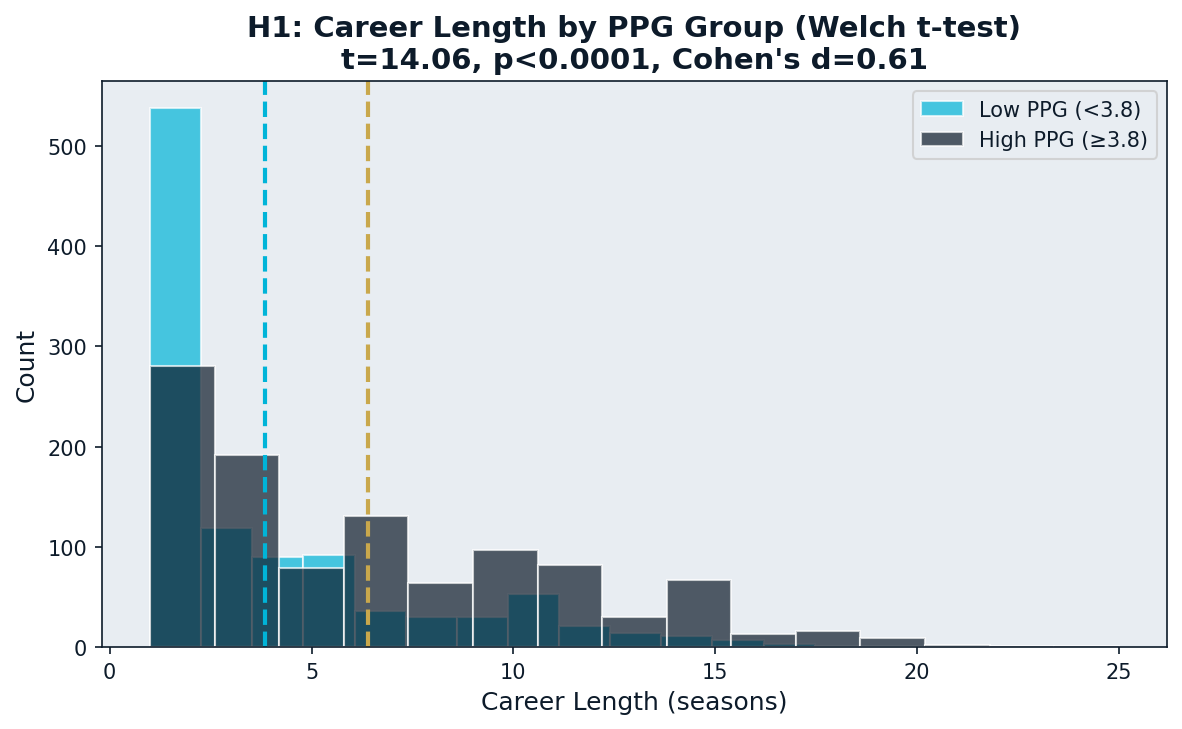
\includegraphics[width=\linewidth]{fig3_h1_ppg.png}
  \caption{Career length by rookie-season PPG group (Welch t-test).}
  \label{fig:h1}
\end{figure}

\begin{figure}[htbp]
  \centering
  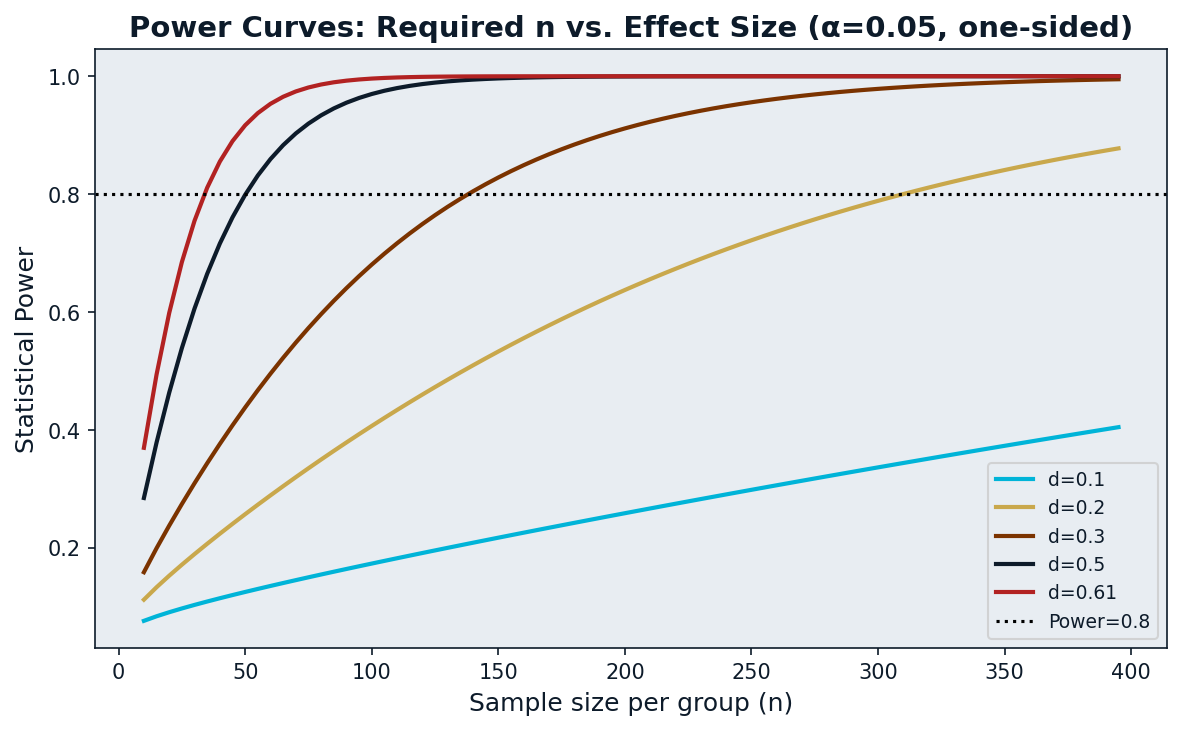
\includegraphics[width=\linewidth]{fig16_power_curve.png}
  \caption{Power curves for the two-sample $t$-test across effect
  sizes, showing the sample size needed to reliably detect smaller
  effects than observed in H1.}
  \label{fig:power}
\end{figure}

\subsection{H2: Draft Round and Career Length}
Mean career length was \textbf{7.49} seasons for Round-1 picks
($n=781$), \textbf{4.38} for Round-2 picks ($n=601$), and
\textbf{3.22} for undrafted players ($n=728$) (Fig.~\ref{fig:h2}).
Levene's test for variance homogeneity ($\mathrm{stat}=87.07$,
$p<0.0001$) indicates the ANOVA equal-variance assumption is
\textbf{violated} --- group variances differ significantly (Round-1
SD$=4.63$ vs.\ Undrafted SD$=3.18$). A one-way ANOVA nonetheless gives
$F=236.8$, $p<0.0001$; more importantly, this is corroborated by the
non-parametric \textbf{Kruskal--Wallis} test ($H=443.4$, $p<0.0001$),
which does not require the equal-variance assumption and is the more
trustworthy result given the Levene violation. Bonferroni-corrected
Welch pairwise comparisons ($\alpha=0.0167$) confirm \textit{all three}
pairs differ significantly (Round~1 vs.\ Round~2: $t=13.73$,
$p<0.0001$; Round~1 vs.\ Undrafted: $t=21.03$, $p<0.0001$; Round~2
vs.\ Undrafted: $t=5.93$, $p<0.0001$). A Chi-square test of
independence between draft group and a three-level career-length
category reinforces this: $\chi^2=370.3$, $df=4$, $p<0.0001$.
\textbf{H2 is strongly supported.}

\begin{figure}[htbp]
  \centering
  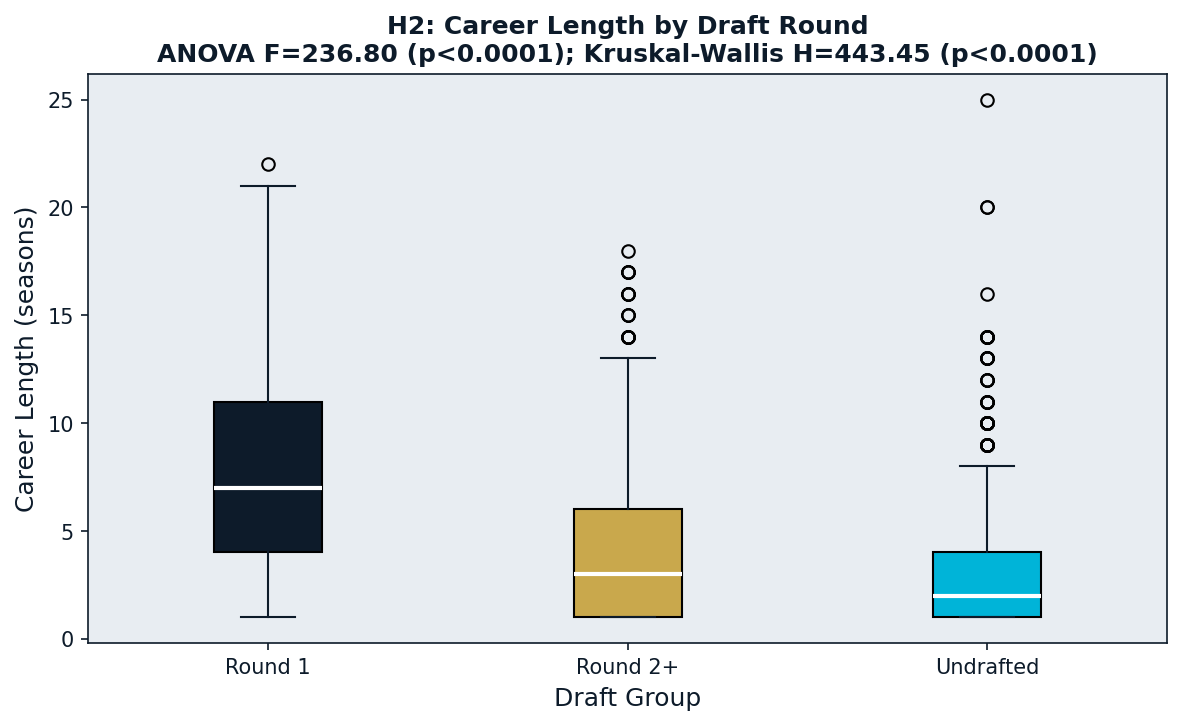
\includegraphics[width=\linewidth]{fig4_h2_draft_round.png}
  \caption{Career length by draft group (ANOVA + Kruskal-Wallis).}
  \label{fig:h2}
\end{figure}

\subsection{H3: Draft Age and Career Length}
Age at a player's first NBA season shows Pearson $r=-0.294$,
$p<0.0001$ (95\% CI $(-0.332,\,-0.254)$), confirmed by Spearman's
$\rho=-0.317$, $p<0.0001$, in the incident-cohort sample. \textbf{Sanity
check:} draft-age SD here is \textbf{2.40} seasons, close to the true
NBA rookie-age SD of $\approx$1.5--1.7 (see
Section~\ref{sec:limitations} for the small residual gap and its
likely cause).

\textbf{Sensitivity check: incident vs.\ prevalent+incident cohort.}
As a robustness check, we repeated this correlation on the full,
unfiltered sample (prevalent + incident cohorts, $n=2{,}551$, i.e.\
including players already active before the dataset's 1996--97 start).
The association is weaker there ($r=-0.210$) than in the incident
cohort alone ($r=-0.294$). This is consistent with \textbf{length-biased
sampling} in the prevalent-cohort component: a cross-sectional data
window over-represents already-established, long-career players among
those whose careers began before the window opened, which dilutes the
observed age--longevity association. We use the incident cohort as our
primary analytic sample throughout this paper for this reason.
Fig.~\ref{fig:h3} shows the incident-cohort relationship (OLS slope
$=-0.53$). \textbf{H3 is supported.}

\begin{figure}[htbp]
  \centering
  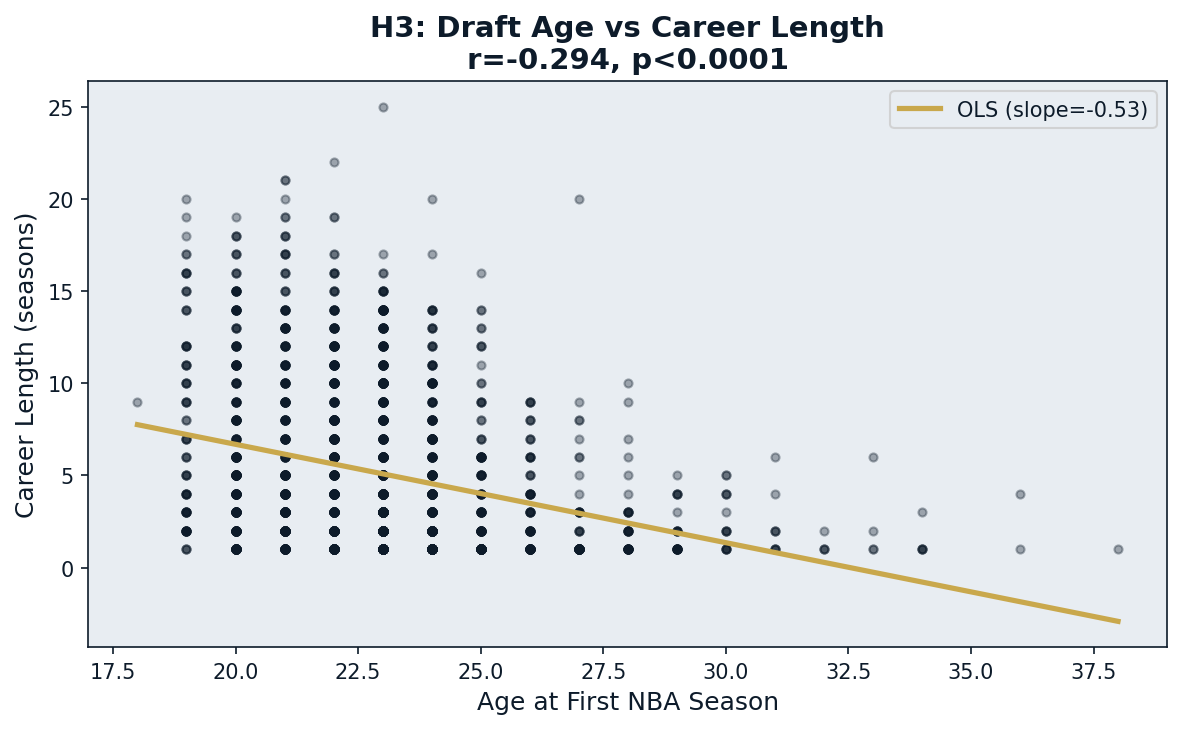
\includegraphics[width=\linewidth]{fig5_h3_age.png}
  \caption{Career length vs.\ age at first NBA season.}
  \label{fig:h3}
\end{figure}

\subsection{Multiple Regression: Combining All Predictors}
We fit an OLS regression of career length on eight standardized
rookie-season predictors (Fig.~\ref{fig:coef}): $R^2=0.203$
(Adj-$R^2=0.200$). Five predictors are significant at $p<0.05$: RPG
($\beta=0.83$), APG ($\beta=0.53$), draft age ($\beta=-0.94$), usage \%
($\beta=0.24$, $p=0.011$), and PPG ($\beta=0.35$, $p=0.047$, only
marginally significant despite its strong univariate H1 effect ---
likely due to collinearity with RPG/APG, $r=0.65$--$0.73$; see
Fig.~\ref{fig:corr}). Net rating narrowly misses significance
($p=0.056$); height/weight are not significant. Draft age remains the
largest-magnitude coefficient, comparable to RPG (see the
incident-cohort sensitivity check in Section~\ref{sec:results}.D for
why this coefficient is not as extreme as it would be on an unfiltered
sample).

\begin{figure}[htbp]
  \centering
  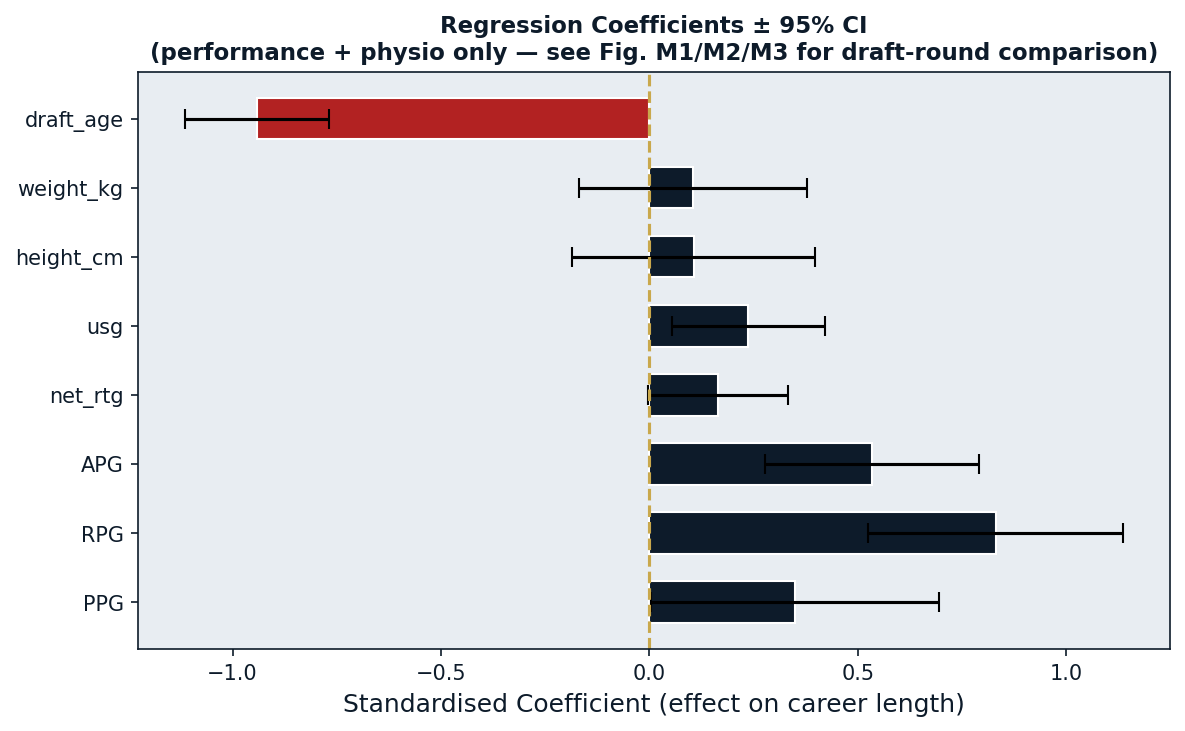
\includegraphics[width=\linewidth]{fig7_coefficients.png}
  \caption{Standardized OLS coefficients (performance + physio only) with 95\% CIs.}
  \label{fig:coef}
\end{figure}

\subsection{H4: Nested Model Comparison --- Rookie Attributes vs.\
Draft Round}
Following \citet{staw1995sunk} and \citet{groothuis2004exit}, we test
whether on-court performance and draft round each carry independent
explanatory power by comparing three nested models
(Fig.~\ref{fig:nested}): \textbf{M1} (rookie-season attributes ---
performance, physical measurements, and draft age together,
$R^2=0.203$), \textbf{M2} (draft group only, $R^2=0.184$), and
\textbf{M3} (both, $R^2=0.251$). The nested $F$-test from M1 to M3 ---
algebraically a Generalized Likelihood Ratio Test for nested linear
models (Section~\ref{sec:methods}) --- tests whether draft group adds
power beyond rookie-season attributes: $F(2,2099)=66.7$, $p<0.0001$
(equivalently, GLRT $-2\log\Lambda=130.0 \sim \chi^2_2$, $p<0.0001$).
The reverse test (M2 to M3) tests whether rookie-season attributes add
power beyond draft group: $F(8,2099)=23.6$, $p<0.0001$. \textbf{Both
directions are highly significant}: rookie-season attributes and
draft round each carry statistically independent explanatory power,
neither subsuming the other. This directly confirms \textbf{H4} and
replicates, on a modern (1997--2022) cohort, the core finding of
\citet{staw1995sunk} and \citet{groothuis2004exit} that draft position
affects career outcomes even after controlling for on-court
performance. Note that M1 already includes draft age alongside
performance and physical measurements; the interaction analysis below
and the regression in the previous subsection isolate the specific
contribution of scoring output (PPG) within this broader set.

\begin{figure}[htbp]
  \centering
  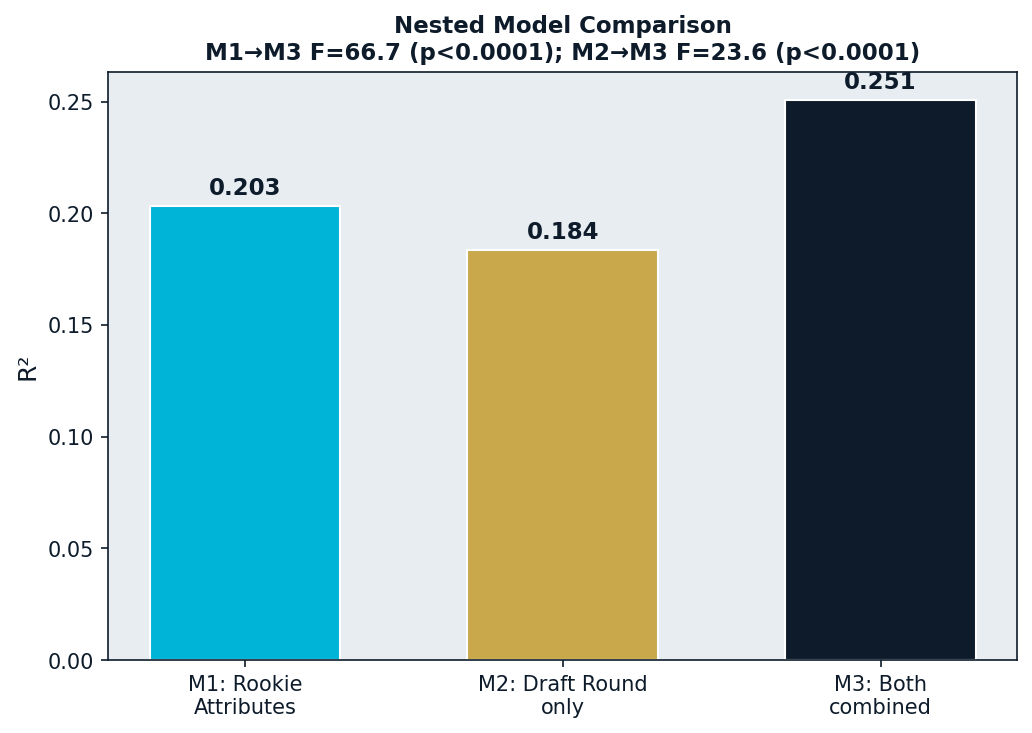
\includegraphics[width=\linewidth]{fig17_nested_models.png}
  \caption{Nested model comparison: $R^2$ for rookie-attributes-only,
  draft-only, and combined models.}
  \label{fig:nested}
\end{figure}

\subsection{Does Performance Compensate for Draft Position? An
Interaction Effect}
Adding an interaction term between rookie PPG and draft group
(Fig.~\ref{fig:interact}) tests whether PPG's effect on career length
depends on draft round. The PPG$\times$Round2+ interaction is
significant ($\beta=0.71$, $p=0.0057$): the slope relating PPG to
career length is steeper for Round-2+ picks than for Round-1 picks.
The PPG$\times$Undrafted interaction is \textbf{not} significant
($\beta=-0.07$, $p=0.77$). We do not interpret this as evidence that
performance fails to help undrafted players reach longer careers ---
only \textbf{30 undrafted players} in the sample have a standardized
PPG above 1 (i.e., reach high scoring output at all), so this cell is
too thin to estimate the interaction precisely. The correct reading is
that our data cannot distinguish a true null effect from a
low-power result for this subgroup, not that performance is proven
irrelevant for undrafted players.

\begin{figure}[htbp]
  \centering
  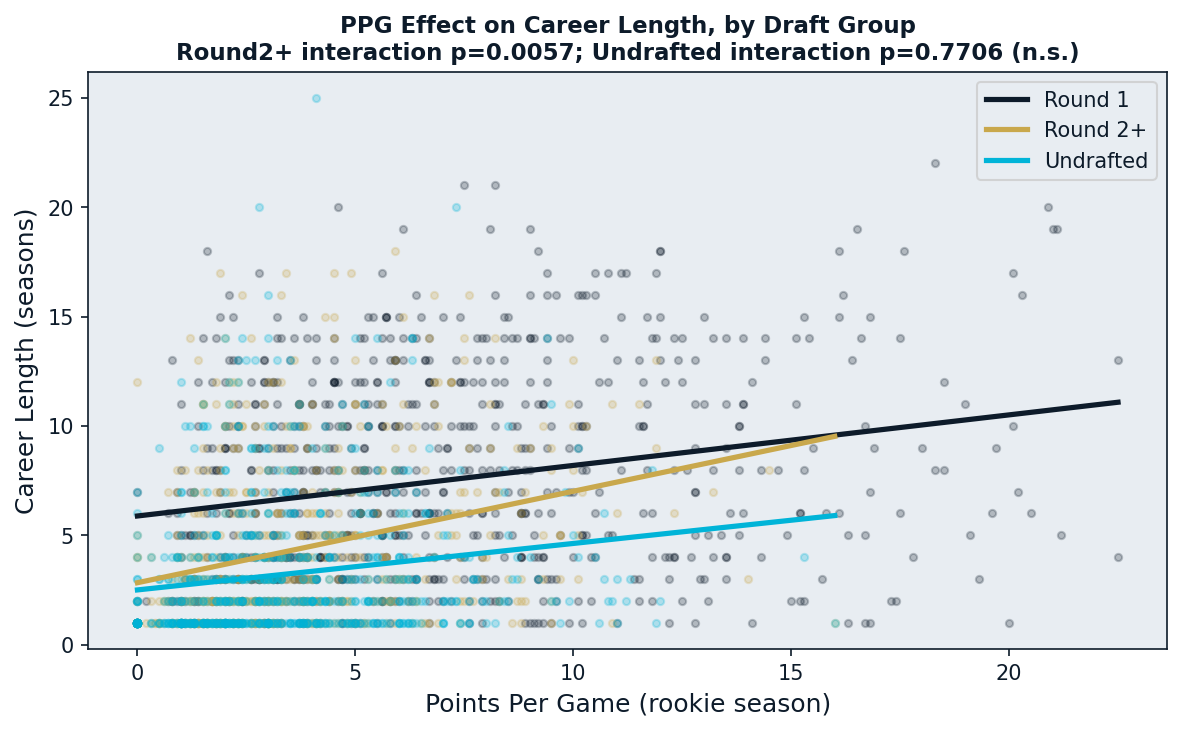
\includegraphics[width=\linewidth]{fig11_interaction.png}
  \caption{Fitted PPG--career length slopes by draft group.}
  \label{fig:interact}
\end{figure}

\subsection{Classification: Predicting Long vs.\ Short Careers}
A logistic regression on the same feature set as M3 (rookie-season
attributes plus draft-group dummies), evaluated on a held-out 25\%
test set, achieved \textbf{66.1\% accuracy} and \textbf{AUC$=0.719$}
(Fig.~\ref{fig:roc}, confusion matrix Fig.~\ref{fig:confusion})
against a \textbf{50.7\%} majority-class baseline (classes were nearly
balanced: 50.7\% Long vs.\ 49.3\% Short) --- a meaningful improvement
over chance, consistent with H4: draft round carries additional,
independent predictive signal beyond performance and physical
attributes alone. All coefficients point in the expected direction:
PPG, RPG, APG, net rating, usage, height, and weight all increase the
odds of a long career; draft age, being drafted in Round~2 or later
($\beta=-0.45$), and going undrafted ($\beta=-0.67$, the largest-
magnitude coefficient in the model) all decrease it.

\begin{figure}[htbp]
  \centering
  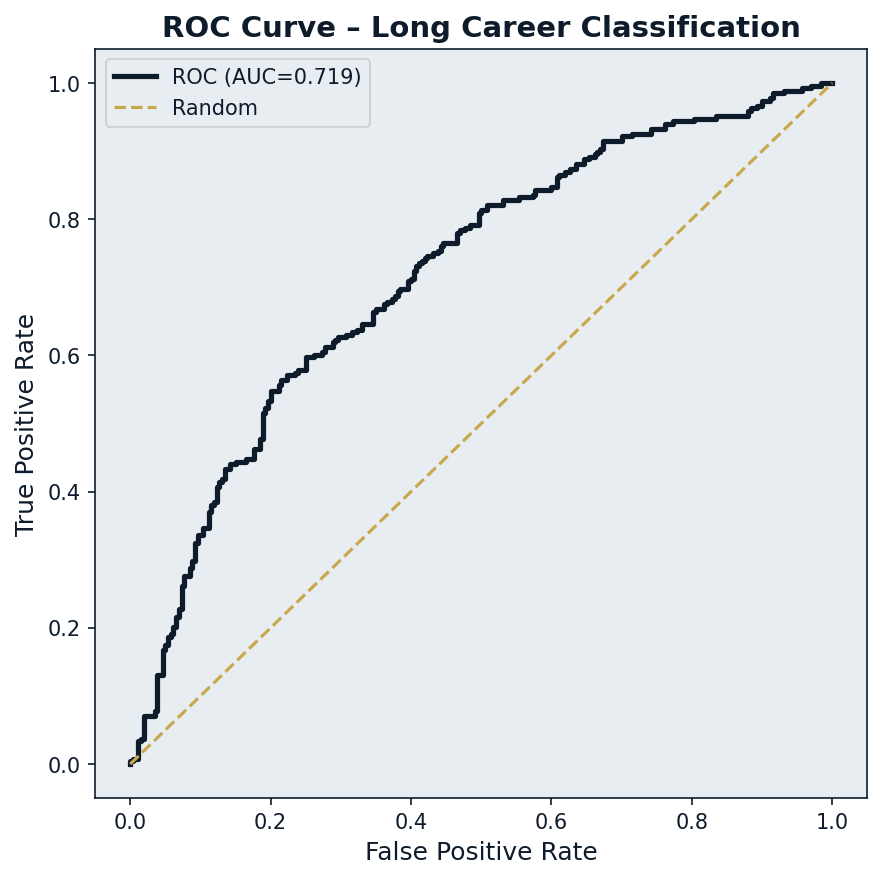
\includegraphics[width=0.49\linewidth]{fig12_roc.png}\hfill
  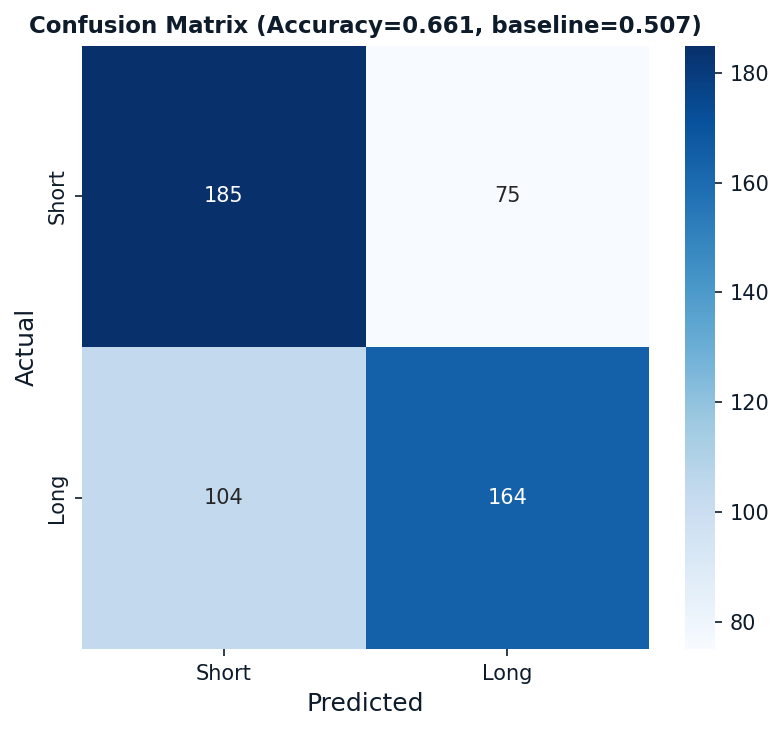
\includegraphics[width=0.49\linewidth]{fig13_confusion.png}
  \caption{Long-vs-Short career classifier (M3 feature set): ROC curve
  (left) and confusion matrix (right).}
  \label{fig:roc}
  \label{fig:confusion}
\end{figure}

\subsection{Model Validation: Cross-Validation}
5-fold cross-validation of \textbf{M3} (rookie-season attributes plus
draft-group dummies --- the paper's headline model, rather than M1
alone) (Fig.~\ref{fig:cv}) gives mean CV $R^2=0.238$ ($\pm0.032$),
compared to in-sample $R^2=0.251$ (matching M3's value in
Section~\ref{sec:results}.G exactly, as expected) --- a gap of only
$0.013$. This small gap indicates the model \textbf{generalizes well}
and is not meaningfully overfit.

\begin{figure}[htbp]
  \centering
  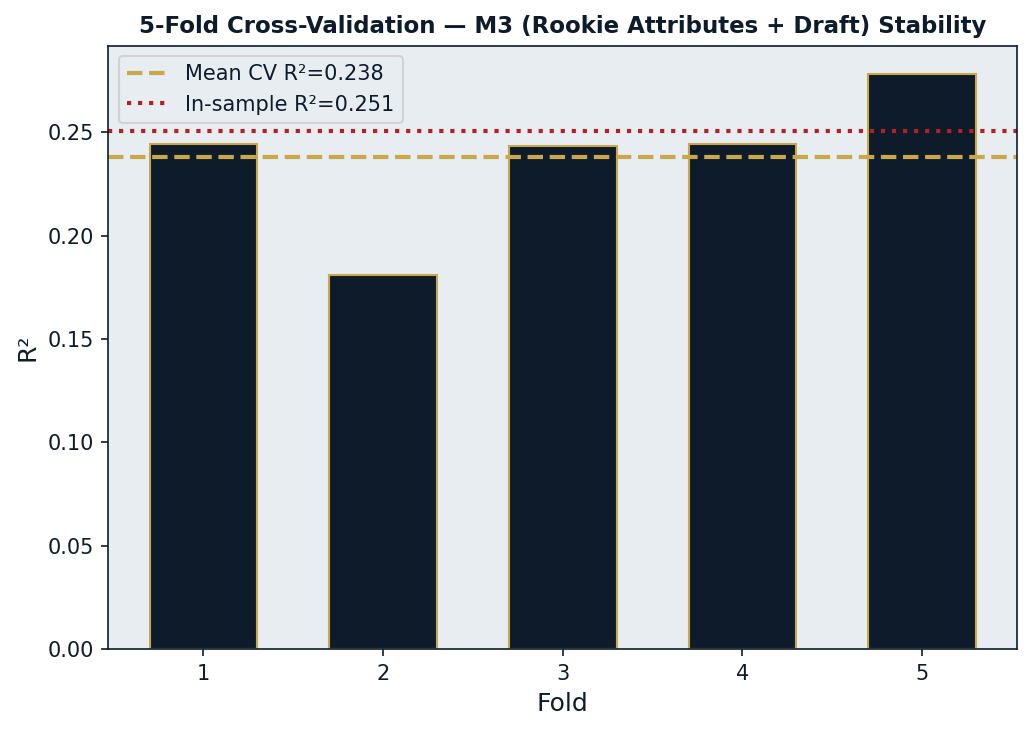
\includegraphics[width=\linewidth]{fig14_crossval.png}
  \caption{5-fold cross-validated $R^2$ vs.\ in-sample $R^2$ for M3.}
  \label{fig:cv}
\end{figure}

\subsection{Sequential Testing: Wald SPRT (1000-Simulation)}
Because a single sequence's stopping decision depends on the order in
which observations arrive, we run the Wald SPRT across 1000
independent random re-orderings of the high-PPG subgroup rather than a
single pass, testing $H_0:\mu=5.13$ (overall mean) against
$H_1:\mu=6.44$ ($0.3\sigma$ above baseline; the subgroup's true mean,
6.39, lies close to $H_1$) (Fig.~\ref{fig:wald}). Across 1000
simulations, the test \textbf{rejects $H_0$ (supports $H_1$) in
77.8\%} of runs and accepts $H_0$ in 22.2\%, with no ``no-decision''
cases, consistent with H1's much larger-sample $t$-test finding above.
The empirical mean stopping time (ASN) is \textbf{48.1} observations
(median 38), reasonably close to Wald's theoretical ASN approximation
of \textbf{42.4}.

\begin{figure}[htbp]
  \centering
  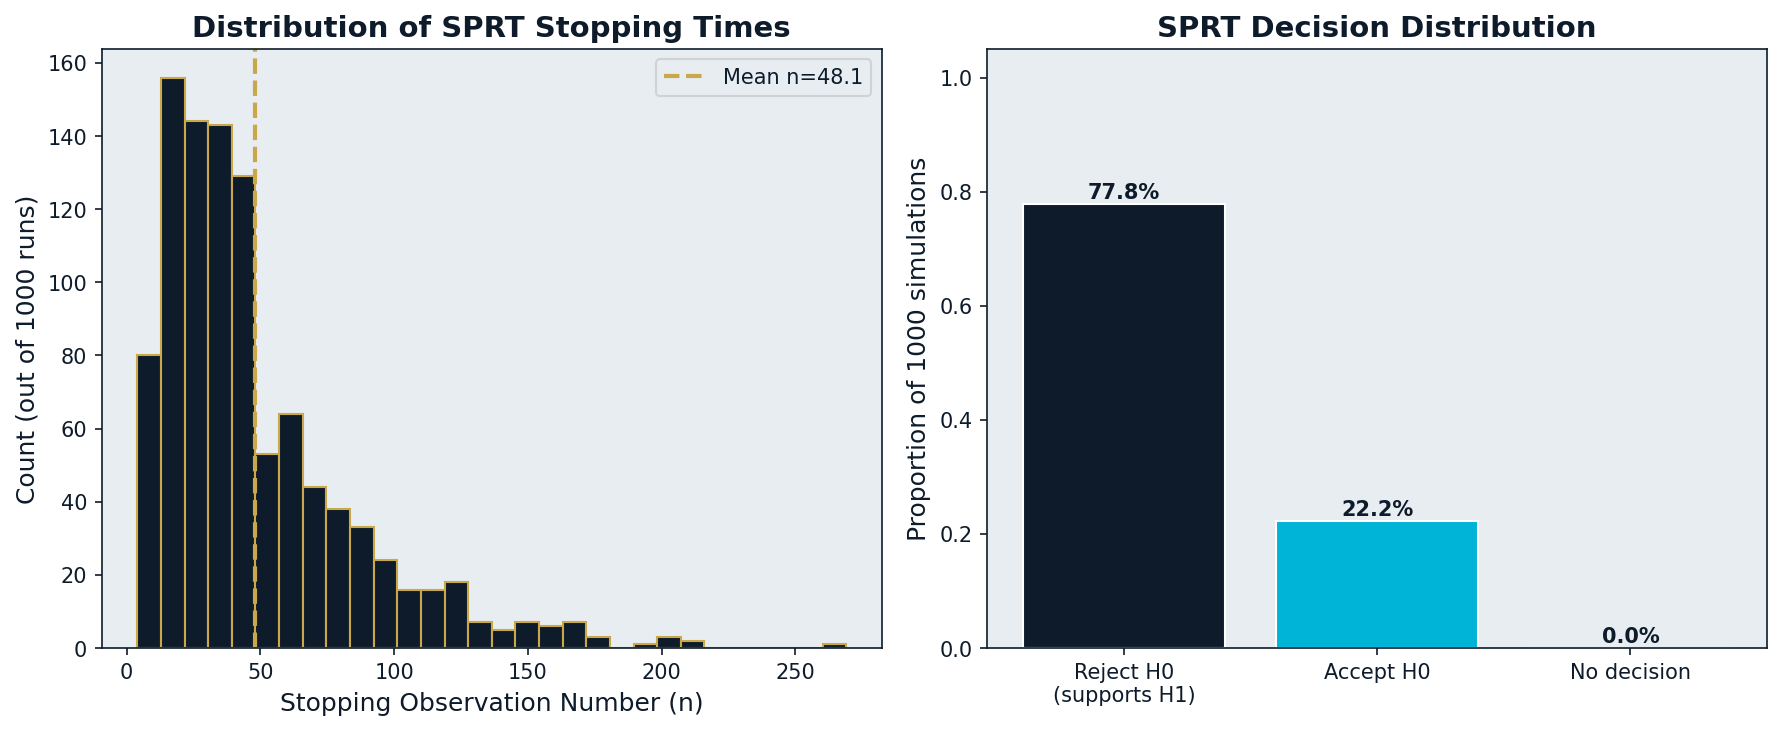
\includegraphics[width=\linewidth]{fig9_wald.png}
  \caption{Distribution of SPRT stopping times and decisions across
  1000 random re-orderings.}
  \label{fig:wald}
\end{figure}

\subsection{Correlation Structure}
Fig.~\ref{fig:corr} summarizes pairwise correlations among key
variables. PPG, RPG, and APG are strongly inter-correlated
($r=0.65$--$0.73$), as expected since high-usage players tend to
accumulate multiple counting statistics simultaneously --- this
collinearity is the most likely explanation for PPG's comparatively
weak, only-marginal significance in the multiple regression
(Fig.~\ref{fig:coef}) despite its strong univariate effect in H1: once
RPG and APG are in the model, PPG has limited additional (non-shared)
variance left to explain. Draft age is negatively correlated with all
three performance statistics, height, and career length itself,
consistent with the H3 and H4 results above.

\begin{figure}[htbp]
  \centering
  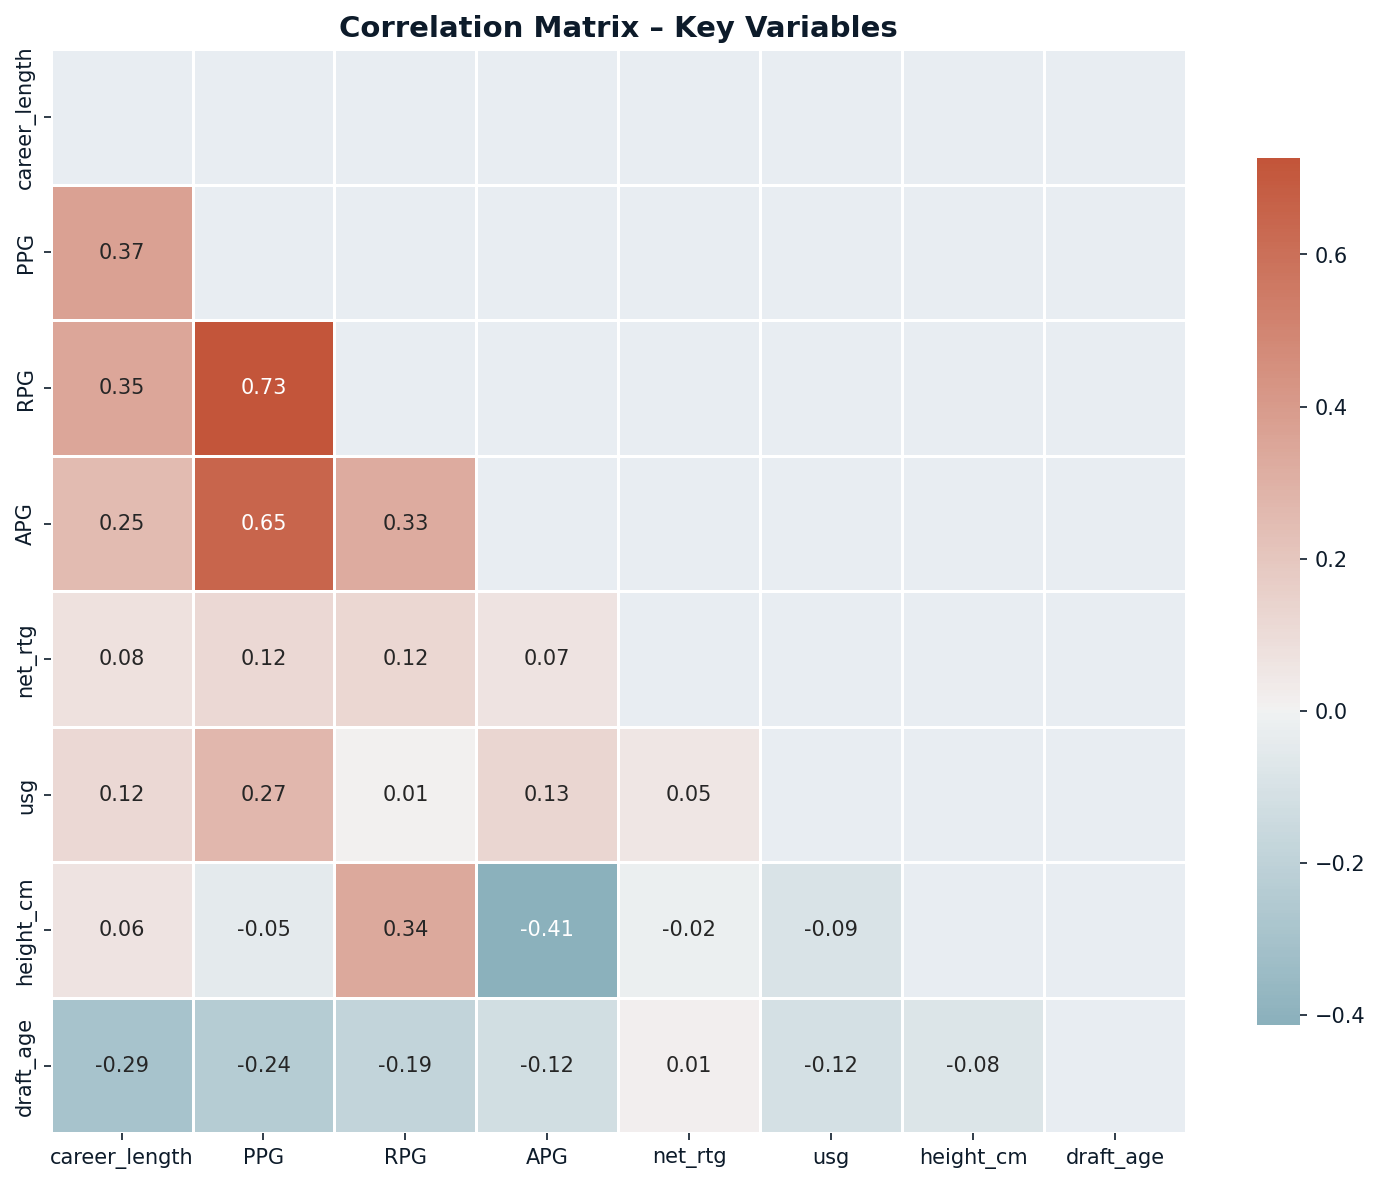
\includegraphics[width=\linewidth]{fig10_correlation.png}
  \caption{Correlation matrix of key variables.}
  \label{fig:corr}
\end{figure}

% ════════════════════════════════════════════════════════════
\section{Methods}
\label{sec:methods}
% ════════════════════════════════════════════════════════════

\subsection{Q-Q Plot}
As a visual complement to the formal goodness-of-fit tests above, we
use a Quantile-Quantile (Q-Q) plot, which plots the sample's ordered
values against the quantiles of a theoretical reference distribution
\citep{wikiqq2024}. Points falling along the $y=x$ reference line
indicate agreement with the reference distribution; systematic curvature
indicates the specific way the sample's distribution departs from it
(e.g.\ heavier tails, skew).

\subsection{Goodness-of-Fit: KS, Shapiro--Wilk, and Discrete $\chi^2$}
The Kolmogorov--Smirnov (KS) test evaluates whether a sample is drawn
from a specified theoretical distribution by comparing the empirical
cumulative distribution function (ECDF) $F_n(x)$ of the sample to the
cumulative distribution function $F(x)$ of the reference distribution:
$D_n = \sup_x | F_n(x) - F(x) |$. A subtlety applies when the reference
distribution's parameters (e.g.\ $\mu,\sigma$) are estimated from the
\textit{same} sample being tested: the standard KS null distribution is
then no longer exact (the Lilliefors problem), so we report KS results
as indicative only. The \textbf{Shapiro--Wilk} test is a more powerful
alternative for detecting non-normality. Because \texttt{career\_length}
is a small positive integer with many tied values, violating KS's
continuity assumption, we treat a \textbf{discrete Pearson $\chi^2$
goodness-of-fit test} as primary: observations are binned into $k$
categories, and
\[
  \chi^2 = \sum_{i=1}^{k} \frac{(O_i - E_i)^2}{E_i} \sim \chi^2_{k-1-m},
\]
where $E_i$ is the expected count in bin $i$ under the reference
distribution and $m$ is the number of parameters estimated from the
data. We apply this both against a Normal reference and against a
\textbf{Geometric distribution} fit by maximum likelihood
($\hat p = 1/\bar{X}$, the natural ``constant season-to-season exit
probability'' model for career length, $P(L=k)=(1-p)^{k-1}p$).

\subsection{Independent-Samples Welch t-test and Mann--Whitney U Test}
To compare mean career length between two independent groups (e.g.,
high- vs.\ low-scoring rookies), we use \textbf{Welch's $t$-test},
which does not assume equal variances between groups:
\[
  t = \frac{\bar{X}_1 - \bar{X}_2}
           {\sqrt{\tfrac{s_1^2}{n_1} + \tfrac{s_2^2}{n_2}}},
\]
where $\bar{X}_i$, $s_i^2$, and $n_i$ are the sample mean, variance, and
size of group $i$; this also matches the standard error used for our
confidence intervals below. We use Welch's version rather than the
equal-variance (Student's) $t$-test because group variances differ
between our draft-round subgroups (confirmed by Levene's test,
Section~\ref{sec:methods}.D). The $t$-test still assumes approximately
normal data; because our goodness-of-fit tests indicate career length
is right-skewed, we pair every $t$-test with the non-parametric
\textbf{Mann--Whitney U test} as a robustness check. The Mann--Whitney
test ranks all observations from both groups together and computes
\[
  U_1 = n_1 n_2 + \frac{n_1(n_1+1)}{2} - R_1,
\]
where $R_1$ is the sum of ranks in group 1 (and $U_2$ analogously for
group 2), testing whether one group tends to produce larger values than
the other without assuming any particular distribution.

\subsection{Effect Size and Statistical Power}
Statistical significance ($p$-value) does not by itself convey the
practical magnitude of a difference, nor the test's ability to detect
one. We report \textbf{Cohen's $d$},
\[
  d = \frac{\bar{X}_1 - \bar{X}_2}{s_{\text{pooled}}}, \qquad
  s_{\text{pooled}} = \sqrt{\frac{s_1^2 + s_2^2}{2}},
\]
which expresses the gap between two group means in units of pooled
standard deviation ($|d|\approx 0.2$, $0.5$, $0.8$: small, medium,
large). We additionally report \textbf{statistical power}: $1-\beta$,
the probability of correctly rejecting $H_0$ when a real effect of a
given size exists, computed exactly via the noncentral $t$-distribution
with noncentrality parameter $\delta = d\sqrt{n/2}$ (equal group
sizes). This connects directly to the trade-off between Type~I error
($\alpha$, falsely rejecting a true $H_0$) and Type~II error ($\beta$,
failing to reject a false $H_0$): for fixed $\alpha$, power increases
with sample size and with the true effect size, which we illustrate
with a power curve across a range of $n$ and $d$ (Fig.~\ref{fig:power}).

\subsection{Variance Homogeneity: Levene's Test, and Kruskal--Wallis}
One-way ANOVA (below) assumes equal variances across groups.
\textbf{Levene's test} checks this by testing whether the group means
of $|X_{ij} - \bar{X}_i|$ (absolute deviations from each group mean)
are themselves equal across groups, via a standard one-way ANOVA on
those deviations; a significant result indicates heteroscedasticity. As
a non-parametric counterpart to ANOVA --- filling the same role
Mann--Whitney fills for the two-sample $t$-test --- we also report the
\textbf{Kruskal--Wallis $H$ test}, which extends the Mann--Whitney
rank-sum idea to more than two groups without assuming equal variances
or normality:
\[
  H = \frac{12}{N(N+1)} \sum_{i=1}^{k} \frac{R_i^2}{n_i} - 3(N+1),
\]
where $R_i$ is the sum of ranks in group $i$ (ranking all $N$
observations together) and $n_i$ is group $i$'s size; under $H_0$,
$H \sim \chi^2_{k-1}$ approximately.

\subsection{One-Way ANOVA and Bonferroni Post-Hoc Correction}
To compare mean career length across more than two groups (Round~1,
Round~2+, and Undrafted players), we use one-way Analysis of Variance
(ANOVA), which tests
$H_0: \mu_1 = \mu_2 = \dots = \mu_k$
via the $F$-statistic, the ratio of between-group to within-group
variance. A significant ANOVA result indicates \textit{at least one}
group differs, but not which, so we follow it with pairwise Welch
$t$-tests, applying the \textbf{Bonferroni correction} (testing each
pair at $\alpha/m$, $m$=number of comparisons) to control the
family-wise error rate (FWER). Our study runs $\approx$25 tests in
total; we apply Bonferroni locally where multiplicity is explicit
(draft-round pairs) and treat any borderline ($0.01<p<0.05$) result
elsewhere with appropriate caution given this broader FWER concern.

\subsection{Correlation: Pearson and Spearman}
To quantify the linear association between two continuous variables
(e.g., draft age and career length), we compute the \textbf{Pearson
correlation coefficient},
\[
  r_{XY} = \frac{\mathrm{Cov}(X,Y)}{\sigma_X \sigma_Y},
\]
together with a 95\% confidence interval obtained via the Fisher
$z$-transformation, $z = \tanh^{-1}(r)$, which is approximately normally
distributed with standard error $1/\sqrt{n-3}$. Because Pearson's $r$
assumes a linear relationship and is sensitive to outliers, we
additionally report \textbf{Spearman's rank correlation} $\rho$, computed
identically to Pearson's $r$ but on the ranks of the data rather than the
raw values, making it robust to monotonic non-linear relationships.

\subsection{Multiple Linear Regression (OLS)}
To model career length as a function of several rookie-season variables
simultaneously, we fit an Ordinary Least Squares (OLS) regression,
\[
  y = X\beta + \varepsilon,
\]
where $y$ is the vector of career lengths, $X$ is the design matrix of
standardized predictors (points, rebounds, and assists per game, net
rating, usage percentage, height, weight, and draft age), and
$\hat\beta = (X^\top X)^{-1} X^\top y$ minimizes the sum of squared
residuals. Model fit is summarized by $R^2 = 1 - \mathrm{SS}_{res} /
\mathrm{SS}_{tot}$, the proportion of variance in career length explained
by the model, and each coefficient's significance is assessed via its
$t$-statistic, $t_j = \hat\beta_j / \mathrm{SE}(\hat\beta_j)$.

\subsection{Nested Model Comparison and the Generalized Likelihood
Ratio Test (GLRT)}
To directly test H4 --- whether rookie-season attributes and draft
round each carry \textit{independent} explanatory power, rather than
one subsuming the other --- we compare three nested OLS models:
rookie-season attributes only (M1: performance, physical measurements,
and draft age), draft-group-only (M2), and both combined (M3). For
nested linear models under normally-distributed errors, the classical
nested $F$-test,
\[
  F = \frac{(\mathrm{SS}_{res,\,reduced} - \mathrm{SS}_{res,\,full})/q}
           {\mathrm{SS}_{res,\,full}/(n-k_{full}-1)} \sim F_{q,\,n-k_{full}-1},
\]
(where $q$ is the number of additional parameters in the full model)
is algebraically equivalent to a \textbf{Generalized Likelihood Ratio
Test (GLRT)} comparing the reduced and full models: the GLRT statistic
$-2\log\Lambda = n\log(\mathrm{SS}_{res,\,reduced}/\mathrm{SS}_{res,\,full})$
is asymptotically $\chi^2_q$-distributed under $H_0$ (reduced model is
adequate), and gives the same substantive conclusion as the $F$-test.
We report both forms. Testing M1$\to$M3 asks whether draft group
improves the model beyond rookie-season attributes alone; testing
M2$\to$M3 asks the reverse.

\subsection{Neyman--Pearson Optimality: MP and UMP Tests}
For simple hypotheses $H_0:\theta=\theta_0$ vs.\ $H_1:\theta=\theta_1$,
the Neyman--Pearson lemma shows the likelihood-ratio test is
\textbf{Most Powerful (MP)} at any significance level --- precisely
the rule underlying the Wald SPRT below, applied sequentially. For the
composite alternative $H_1:\mu>\mu_0$ used in our $t$-tests, the
one-sided $t$-test is \textbf{Uniformly Most Powerful (UMP)} among
unbiased tests. This is why $t$-tests (and their Welch variant) are our
primary tool for directional hypotheses, with Mann--Whitney as a
distribution-free check.

\subsection{Regression with Interaction Terms}
A purely additive regression assumes each predictor's effect on career
length is constant regardless of the other predictors' values. To test
whether the effect of rookie PPG on career length \textit{depends} on
draft round, we extend the model with an interaction term,
\[
  y = \beta_0 + \beta_1 \mathrm{PPG} + \beta_2 D + \beta_3 (\mathrm{PPG}
  \times D) + \varepsilon,
\]
where $D$ is a dummy variable for draft group. A significant $\beta_3$
indicates that the slope relating PPG to career length differs across
draft groups --- for example, that strong rookie performance compensates
more for a low draft position than for a high one, or vice versa.

\subsection{Chi-Square Test of Independence}
To test whether two categorical variables (draft group and a
career-length category of Short/Medium/Long) are statistically
independent, we construct a contingency table of observed counts $O_{ij}$
and compute
\[
  \chi^2 = \sum_{i,j} \frac{(O_{ij} - E_{ij})^2}{E_{ij}},
\]
where $E_{ij}$ is the expected count under independence. A large $\chi^2$
relative to its degrees of freedom (and correspondingly small $p$-value)
indicates the two variables are associated rather than independent.

\subsection{Wald Sequential Probability Ratio Test (SPRT)}
Unlike the fixed-sample tests above, the Wald Sequential Test evaluates
evidence \textit{as observations arrive}, stopping as soon as enough
evidence has accumulated to decide between two simple hypotheses
$H_0: \mu = \mu_0$ and $H_1: \mu = \mu_1$ (by the Neyman--Pearson/MP
argument above, the per-step log-likelihood-ratio is the optimal
statistic to accumulate). For two Normal distributions with common
variance $\sigma^2$, the exact per-observation increment is
\[
  \log\frac{f(x\mid H_1)}{f(x\mid H_0)}
  = \frac{\mu_1-\mu_0}{\sigma^2}\,x \;-\; \frac{\mu_1^2-\mu_0^2}{2\sigma^2},
\]
and the cumulative sum $\Lambda_n=\sum_{i=1}^n \log[f(x_i\mid H_1)/f(x_i\mid H_0)]$
is compared against two boundaries, $A = \log\!\big(\tfrac{1-\beta}{\alpha}\big)$
and $B = \log\!\big(\tfrac{\beta}{1-\alpha}\big)$, determined by the
desired Type~I error rate $\alpha$ and Type~II error rate $\beta$.
Sampling stops and $H_0$ is rejected once $\Lambda_n \geq A$, or accepted
once $\Lambda_n \leq B$; otherwise, sampling continues. Because a
single sequence's stopping point depends on the order in which
observations arrive, we run the procedure across 1000 independent
random re-orderings of the data and report the distribution of
decisions and stopping times, together with Wald's classical
approximation for the Average Sample Number (ASN),
$\mathrm{E}[N\mid H_1] \approx \big[(1-\beta)A + \beta B\big] /
\mathrm{E}_{H_1}[\log(f(x\mid H_1)/f(x\mid H_0))]$, as a theoretical
cross-check on the empirical mean stopping time.

\subsection{Logistic Regression for Classification}
To predict a binary outcome --- whether a player's career is
\textit{Long} (at or above the median career length) or \textit{Short}
--- we use logistic regression, which models the log-odds of the
positive class as a linear function of the predictors,
\[
  \log \frac{P(y=1 \mid X)}{1 - P(y=1 \mid X)} = X\beta.
\]
Coefficients are estimated by maximum likelihood. Model performance is
evaluated on a held-out test set (25\% of players, stratified by class)
using \textbf{accuracy}, the proportion of correctly classified
players, compared against the \textbf{majority-class baseline} (the
accuracy achievable by always predicting the more common class ---
the correct comparison point, rather than a naive 50\%, whenever
classes are not perfectly balanced); the \textbf{confusion matrix},
cross-tabulating predicted vs.\ actual class; and the \textbf{ROC
curve} and its area under the curve (\textbf{AUC}), which summarize
the trade-off between true- and false-positive rates across all
classification thresholds. An AUC of 0.5 indicates no better than
random guessing, while 1.0 indicates perfect separation.

\subsection{$k$-Fold Cross-Validation}
Reporting $R^2$ from a model fit and evaluated on the same data risks
overstating performance due to overfitting. We therefore assess
generalizability with $k$-fold cross-validation ($k=5$): the data is
randomly partitioned into five equal folds; the model is trained on four
folds and evaluated on the held-out fifth, repeated so that each fold
serves as the test set exactly once. The five resulting $R^2$ values are
averaged, and a large gap between in-sample $R^2$ and mean
cross-validated $R^2$ signals overfitting.

% ════════════════════════════════════════════════════════════
\section{Discussion}
\label{sec:discussion}
% ════════════════════════════════════════════════════════════

All four hypotheses were supported. Rookie-season scoring (H1) and
draft round (H2) both showed large, highly significant effects; age at
entry (H3) showed a smaller but robust effect; and, critically, H4
confirms performance and draft round each carry \textbf{independent}
explanatory power (nested $F$-tests, both $p<0.0001$) --- neither
subsumes the other. Rather than asking which single factor ``wins'' in
isolation, H4 shows both matter \textit{jointly}, replicating
\citet{staw1995sunk} and \citet{groothuis2004exit} on a modern cohort.

The interaction result adds a nuance worth stating carefully: strong
rookie scoring predicts a steeper career-length benefit for Round-2+
picks than Round-1 picks ($p=0.0057$), but we found no significant
interaction for undrafted players ($p=0.77$) --- not because
performance is irrelevant for them, but because only 30 undrafted
players in our sample reach high rookie PPG, leaving too little data
to estimate that interaction precisely. This distinction (a genuine
null vs.\ a low-power result) should not be glossed over.

Model validation supports these conclusions: the small gap between
M3's in-sample and cross-validated $R^2$ (0.251 vs.\ 0.238) indicates
the regression is not meaningfully overfit, and the M3-feature-set
classifier's 66.1\% accuracy against a 50.7\% majority-class baseline
(AUC$=0.719$) confirms that rookie-season attributes and draft-group
information together carry genuine predictive signal.

\subsection{Limitations}
\label{sec:limitations}
The most significant remaining limitation is \textbf{right-censoring}:
players whose careers were still active near the end of the dataset's
coverage (the 2021--22 season) have their career length recorded as if
it were already final, when in reality their careers may have
continued beyond the data's collection window. This affects
recently-drafted players disproportionately and likely biases their
career-length estimates downward. Standard OLS and logistic regression,
as used here, do not account for this censoring; this is distinct from,
though related to, the left-truncation issue corrected above (which
concerned careers starting \textit{before} the data window, whereas
censoring concerns careers continuing \textit{after} it).

A second limitation is that the regression explains only a modest
share of the variance in career length, meaning most of what
determines how long a player's career lasts --- injuries, coaching
decisions, team context, contract structure, and opportunity variance
--- is not captured by our rookie-season variables.

A third limitation is \textbf{residual left-truncation}: draft-age SD
in our incident cohort (2.40) is close to the true NBA rookie-age
range ($\approx$1.5--1.7) but not fully there --- our filter only
excludes players whose first recorded row is the dataset's first
season, missing players who took a multi-year gap before re-entering.
A stricter filter cross-referencing \texttt{draft\_year} (already
present in the raw data) could resolve this fully. Finally, players
are merged by \texttt{player\_name} (no unique ID exists); we found no
evidence of name-collisions, but note it as a data-quality caveat.

\subsection{Future Work}
The censoring issue above points naturally toward \textbf{survival
analysis} as the statistically appropriate framework for this
question: methods such as the Kaplan--Meier estimator or a Cox
proportional-hazards model are explicitly designed to handle
right-censored time-to-event data, and would allow still-active
players' careers to be included without treating their current career
length as final. Our empirical hazard curve (Fig.~\ref{fig:hazard})
already points in this direction directly: its U-shaped pattern ---
elevated exit risk in the first 1--2 seasons, a mid-career trough
around seasons 5--7, and rising risk again in the later seasons ---
suggests distinct underlying mechanisms at different career stages
(unproven rookies being cut early vs.\ aging veterans retiring late),
which a full Kaplan--Meier estimate would characterize more
rigorously, with proper handling of the right-censored (still-active)
players our current analysis excludes.
Beyond this: a stricter incident-cohort filter using
\texttt{draft\_year} could resolve the residual left-truncation noted
above, and the GLRT comparison could extend to a three-way
decomposition isolating physical attributes separately.

% ════════════════════════════════════════════════════════════
\bibliographystyle{plainnat}
\setlength{\bibsep}{2pt}
\begin{thebibliography}{9}
\scriptsize

\bibitem{sleeper2024draft}
Sleeper Staff, ``NBA Draft: How It Works, When It Is, How Many Rounds
There Are and More,'' \textit{Sleeper}, 2024. [Online]. Available:
\url{https://sleeper.com/blog/how-many-draft-rounds-in-nba/}

\bibitem{kaggle2024nbadata}
J.~Justinas, ``NBA Players Data,'' \textit{Kaggle}, 2023. [Online].
Available: \url{https://www.kaggle.com/datasets/justinas/nba-players-data}

\bibitem{wikiqq2024}
Wikipedia, ``Q--Q plot,'' 2024. [Online]. Available:
\url{https://en.wikipedia.org/wiki/Q-Q_plot}

\bibitem[Staw and Hoang(1995)]{staw1995sunk}
B.~M.~Staw and H.~Hoang, ``Sunk costs in the NBA: Why draft order
affects playing time and survival in professional basketball,''
\textit{Administrative Science Quarterly}, vol.~40, no.~3, pp.~474--494,
1995.

\bibitem[Groothuis and Hill(2004)]{groothuis2004exit}
P.~A.~Groothuis and J.~R.~Hill, ``Exit discrimination in the NBA: A
duration analysis of career length,'' \textit{Economic Inquiry},
vol.~42, no.~2, pp.~341--349, 2004.

\bibitem[Fynn and Sonnenschein(2012)]{fynn2012analysis}
K.~D.~Fynn and M.~Sonnenschein, ``An analysis of the career length of
professional basketball players,'' \textit{The Macalester Review},
vol.~2, no.~2, Article~3, 2012.

\end{thebibliography}

\end{document}
